
%(BEGIN_QUESTION)
% Copyright 2012, Tony R. Kuphaldt, released under the Creative Commons Attribution License (v 1.0)
% This means you may do almost anything with this work of mine, so long as you give me proper credit

Examine this process trend showing the PV, SP, and Output of a loop controller:

$$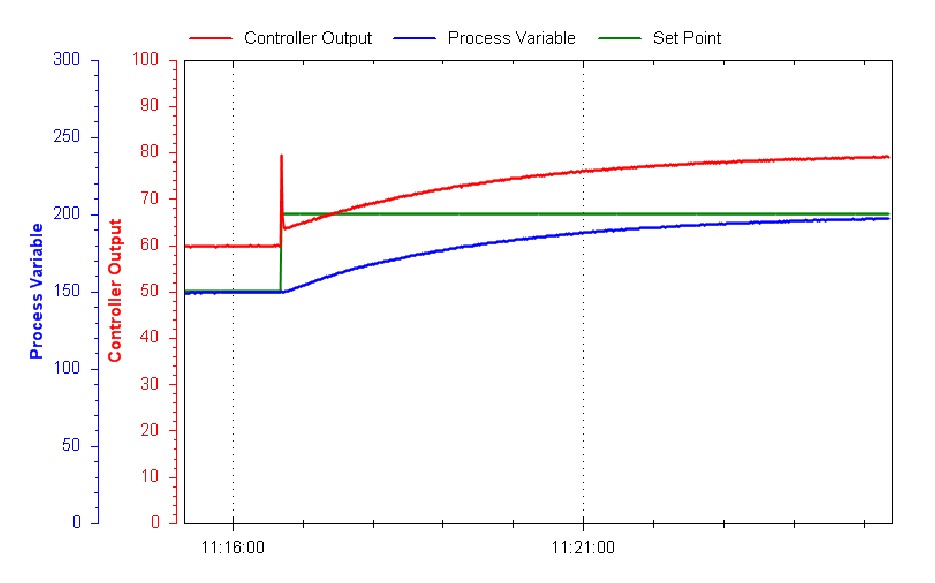
\includegraphics[width=15.5cm]{i01927x01.eps}$$

Based on what you see here, determine the following:

\begin{itemize}
\item{} Whether this is an open-loop or a closed-loop response
\item{} Whether the controller is (or needs to be) {\it direct-acting} or {\it reverse-acting}
\item{} If possible, identify any problems with the field instrumentation
\item{} If possible, identify any problems with the controller PID tuning
\item{} Qualitatively identify the kind of PID tuning we will need for robust control
\end{itemize}

\underbar{file i01927}
%(END_QUESTION)





%(BEGIN_ANSWER)

This is a {\it closed-loop test}, based on the fact the output signal responds dynamically to the changing process variable, as well as to the step-change in setpoint.

\vskip 10pt

This is a {\it reverse-acting} controller: the output steps up when the setpoint steps up (implying the output would step down if the process variable stepped up).

\vskip 10pt

We really cannot discern any problems with field instrumentation from this trend.  A manual-mode (open-loop) test would be more informative in that regard.

\vskip 10pt

The response to the setpoint change shows some derivative action (as seen from the ``spike''), a small amount of proportional action (as seen from the ``step'' of about 4\% following the derivative spike), and a slow integral time.  Integral action is the most challenging to see in this trend, as it looks almost like a proportional response: the long, inverse-exponential curve of the output that has the same shape and magnitude as the process variable's inverse-exponential curve toward setpoint.  We can tell for sure that this is integral action rather than proportional action from the direction of its action: the output is driving up as the process variable continues to be below setpoint (this is reverse action, integral).

\vskip 10pt

More gain (more aggressive proportional action) would probably help, and we could do with faster integral action as well.  Less derivative action might even be helpful here, as its present level could be acting to slow down the response of the controller.

%(END_ANSWER)





%(BEGIN_NOTES)


%INDEX% Control, PID tuning: step change (output) revealing poor controller tuning
%INDEX% Process troubleshooting: diagnosing problem via trend recording

%(END_NOTES)


